\section{Citizens}
	\subsection{Registration}
	If you want to create a personal account for \textit{Soldino} visit the
	homepage and make sure that the slider in set on "Citizen".\\
	\begin{figure}[H]
		
\includegraphics[width=5cm]{res/images/user_citizen.png}
		\centering
		\caption{Select "Citizen" from the slider}
	\end{figure}	
	Then, insert your data in the form. After you have completed all the
	fields with your informations press the "Sign up" button. If an entry 
	is not valid (i.e. the email address does not contain a valid domain) 
	the system will let you know an you must correct that field to continue.
	If all the informations are correct you'll be redirected to a page 
	congratulating you for your registration on the platform.
	\begin{figure}[H]
		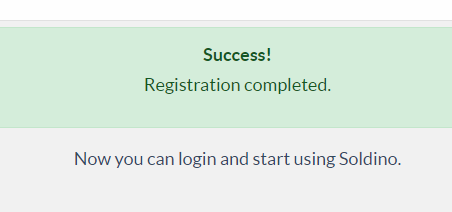
\includegraphics[width=5cm]{res/images/registration_complete.png}
		\centering
		\caption{Registration completed message}
	\end{figure}
	\subsubsection{Citizen already registered}
	If your address is already registered in our platform you will see an
	error page telling you that you cannot create a new account.
	\subsection{Login}
	If you already have a personal account press the "login" button on the 
	top right of the page to be able to buy goods and services or check your
	orders. To be able to login you must be logged in your MetaMask account.
	\subsection{Searching}
	%PLACEHOLDER se viene implementata la ricerca
	\subsection{Buying}
	After you login you will be able to explore the products that 
	\textit{Soldino} has to offer you. If you something you want you
	just have to select the quantity and then press the "Add to cart" button 
	to put it in your cart.
	\subsubsection{Cart}
	After you are done searching for what you need just press the cart icon to
	go to your cart. Here you will find every item you have selected in the 
	respective quantity and above them you will see the total for your order.
	If you need to modify the quantity press the "+" or "-" buttons. \\
	When you want to proceed with the order press the "Checkout" button, 
	you will be redirected to the checkout page
	\subsubsection{Checkout}
	%PLACEHOLDER scrivere qualcosa pagina checout appena viene fatta